\chapter{Proverb 10}

\begin{figure}
  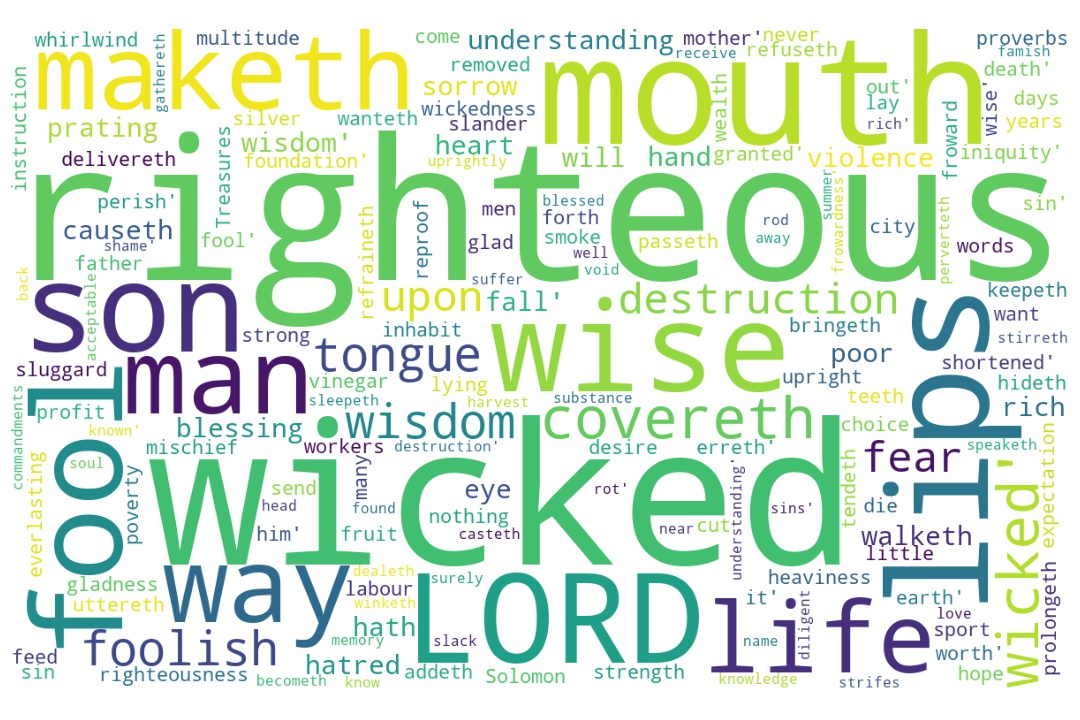
\includegraphics[width=\linewidth]{20OT-Proverbs/Proverb10-WordCloud.jpg}
  \caption{Proverb 10 Word Cloud}
  \label{fig:Proverb 10 Word Cloud}
\end{figure}

\marginpar{\scriptsize \centering\fcolorbox{bone}{lime}{\textbf{THE RIGHTEOUS \& WICKED}}\\ (Proverb 10:1-32)
\begin{compactenum}[I.][8]
	\item \textbf{Shame to the Lazy}  \index[scripture]{Proverbs!Pro 10:05} (Pro 10:5)
	\item \textbf{Sure Footing for the Upright}  \index[scripture]{Proverbs!Pro 10:09} (Pro 10:9)
	\item \textbf{Strife to the Hateful}  \index[scripture]{Proverbs!Pro 10:12} (Pro 10:12)
	\item More \textbf{Sin for the Wicked}  \index[scripture]{Proverbs!Pro 10:16} (Pro 10:16)
	\item \textbf{Sustenance form the Righteous}  \index[scripture]{Proverbs!Pro 10:21} (Pro 10:21)
	\item \textbf{Stinging Eyes to the Sluggard}  \index[scripture]{Proverbs!Pro 10:26} (Pro 10:26)
	\item \textbf{Strength to the Upright} \index[scripture]{Proverbs!Pro 10:29} (Pro 10:29)
\end{compactenum}}

\marginpar{\scriptsize \centering\fcolorbox{bone}{yellow}{\textbf{7 THINGS OF LIFE}}\\ (Proverb 10:1-32)
    \begin{compactenum}[I.][8]
	\item The \textbf{Well} of Life \index[scripture]{Proverbs!Pro 10:11} (Pro 10:11)
	
	\item A \textbf{Wellspring} of Life \index[scripture]{Proverbs!Pro 16:22} \index[scripture]{Proverbs!Pro 18:4} (Pro 16:22, 18:4)
	
	\item The \textbf{way} of Life \index[scripture]{Pro!Pro 06:23} \index[scripture]{Pro!Pro 10:17} \index[scripture]{Pro!Pro 15:24} \index[scripture]{Jer!Jer 21:8} (Pro 6:23, 10:17, 15:24, Jer 21:8)

	\item The \textbf{ways} of Life \index[scripture]{Acts!Acts 02:28} (Acts 2:28)
	
	\item The \textbf{water} of Life \index[scripture]{Rev!Rev 21:06} \index[scripture]{Rev!Rev 22:01} \index[scripture]{Rev!Rev 22:17}  (Rev 21:6, 22:1, 22:17)
	
	\item The \textbf{word} of Life \index[scripture]{Phil!Phil 02:16} (Phil 2:16)
	
	\item The \textbf{Word} of Life \index[scripture]{1Jn!1Jn 1:1}  (1 John 1:1)
\end{compactenum}}

\footnote{\textcolor[cmyk]{0.99998,1,0,0}{\hyperlink{TOC}{Return to end of Table of Contents.}}}\footnote{\href{https://audiobible.com/bible/proverbs_10.html}{\textcolor[cmyk]{0.99998,1,0,0}{Proverbs Audio}}}\textcolor[cmyk]{0.99998,1,0,0}{The proverbs of Solomon. A wise son maketh a glad father: but a foolish son \emph{is} the heaviness of his mother.}
[2] \textcolor[cmyk]{0.99998,1,0,0}{Treasures of wickedness profit nothing: but \fcolorbox{bone}{MYGOLD}{righteousness} delivereth from death.}
[3] \textcolor[cmyk]{0.99998,1,0,0}{The LORD will not suffer the soul of the righteous to famish: but he casteth away the substance of the wicked.}\footnote{\textbf{Psalm 37:25} - I have been young, and now am old; yet have I not seen the righteous forsaken, nor his seed begging bread.}
[4] \textcolor[cmyk]{0.99998,1,0,0}{He becometh poor that dealeth \emph{with} a slack hand: but the hand of the diligent maketh rich.}
[5] \textcolor[cmyk]{0.99998,1,0,0}{He that gathereth in summer \emph{is} a wise son: \emph{but} he that sleepeth in harvest \emph{is} a son that causeth \fcolorbox{bone}{lime}{shame}.}
[6] \textcolor[cmyk]{0.99998,1,0,0}{Blessings \emph{are} upon the head of the just: but violence covereth the mouth of the wicked.}
[7] \textcolor[cmyk]{0.99998,1,0,0}{The memory of the just \emph{is} blessed: but the name of the wicked shall rot.}
[8] \textcolor[cmyk]{0.99998,1,0,0}{Thewise in heart will receive commandments: but a prating fool shall fall.}
[9] \textcolor[cmyk]{0.99998,1,0,0}{He that walketh uprightly walketh \fcolorbox{bone}{lime}{surely}: but he that perverteth his ways shall be known.}
[10] \textcolor[cmyk]{0.99998,1,0,0}{He that winketh with the eye causeth sorrow: but a prating fool shall fall.}\footnote{\textbf{Proverbs 6:13} - He winketh with his eyes, he speaketh with his feet, he teacheth with his fingers;} 
[11] \textcolor[cmyk]{0.99998,1,0,0}{The mouth of a righteous \emph{man} \emph{is} a well of life: but violence covereth the mouth of the wicked.}\footnote{\textbf{Proverb 16:22} - Understanding is a wellspring of life unto him that hath it: but the instruction of fools is folly.}
[12] \textcolor[cmyk]{0.99998,1,0,0}{Hatred stirreth up \fcolorbox{bone}{lime}{strifes}: but love covereth all sins.}
[13] \textcolor[cmyk]{0.99998,1,0,0}{In  the lips of him that hath \fcolorbox{bone}{MYGOLD}{understanding} wisdom is found: but a rod \emph{is} for the back of him that is void of \fcolorbox{bone}{MYGOLD}{understanding}.}
[14] \textcolor[cmyk]{0.99998,1,0,0}{Wise  \emph{men} lay up knowledge: but the mouth of the foolish \emph{is} near destruction.}
[15] \textcolor[cmyk]{0.99998,1,0,0}{The  rich man's wealth \emph{is} his strong city: the destruction of the poor \emph{is} their poverty.}
[16] \textcolor[cmyk]{0.99998,1,0,0}{The  labour of the righteous \emph{tendeth} to life: the fruit of the wicked \fcolorbox{bone}{lime}{to sin}.}
[17] \textcolor[cmyk]{0.99998,1,0,0}{He  \emph{is} \emph{in} the way of life that keepeth instruction: but he that refuseth reproof erreth.}
[18] \textcolor[cmyk]{0.99998,1,0,0}{He  that hideth hatred \emph{with} lying lips, and he that uttereth a slander, \emph{is} a fool.}
[19] \textcolor[cmyk]{0.99998,1,0,0}{In  the multitude of words there wanteth not sin: but he that refraineth his lips \emph{is} wise.}
[20] \textcolor[cmyk]{0.99998,1,0,0}{The tongue of the just \emph{is} \emph{as} choice silver: the heart of the wicked \emph{is} little worth.}
[21] \textcolor[cmyk]{0.99998,1,0,0}{The lips of the righteous \fcolorbox{bone}{lime}{feed many}: but fools die for want of wisdom.}
[22] \textcolor[cmyk]{0.99998,1,0,0}{The blessing of the LORD, it maketh rich, and he addeth no sorrow with it.}
[23] \textcolor[cmyk]{0.99998,1,0,0}{\emph{It} \emph{is} as sport to a fool to do mischief: but a man of \fcolorbox{bone}{MYGOLD}{understanding} hath wisdom.}
[24] \textcolor[cmyk]{0.99998,1,0,0}{The fear of the wicked, it shall come upon him: but the desire of the righteous shall be granted.}
[25] \textcolor[cmyk]{0.99998,1,0,0}{As the whirlwind passeth, so \emph{is} the wicked no \emph{more}: but the righteous \emph{is} an everlasting foundation.}
[26] \textcolor[cmyk]{0.99998,1,0,0}{As vinegar to the teeth, and as \fcolorbox{bone}{lime}{smoke to the eyes}, so \emph{is} the sluggard to them that send him.}
[27] \textcolor[cmyk]{0.99998,1,0,0}{The fear of the LORD prolongeth days: but the years of the wicked shall be shortened.}
[28] \textcolor[cmyk]{0.99998,1,0,0}{The hope of the righteous \emph{shall} \emph{be} gladness: but the expectation of the wicked shall perish.}
[29] \textcolor[cmyk]{0.99998,1,0,0}{The way of the LORD \emph{is} \fcolorbox{bone}{lime}{strength to the upright}: but destruction \emph{shall} \emph{be} to the workers of iniquity.}
[30] \textcolor[cmyk]{0.99998,1,0,0}{The righteous shall never be removed: but the wicked shall not inhabit the earth.}
[31] \textcolor[cmyk]{0.99998,1,0,0}{The mouth of the just bringeth forth wisdom: but the froward tongue shall be cut out.}
[32] \textcolor[cmyk]{0.99998,1,0,0}{The lips of the righteous know what is acceptable: but the mouth of the wicked \emph{speaketh} frowardness.}

